\begin{flushright} {\tiny {\color{gray} openbc.tex}} \end{flushright}
%~~~~~~~~~~~~~~~~~~~~~~~~~~~~~~~~~~~~~~~~~~~~~~~~~~~~~~~~~~~~~~~~~~~~~~~~~~~~~~~~~~~~~~~~~~~~~~~~~~

So-called open boundary conditions have a special meaning in computational geodynamics. 
They usually refer to the boundary conditions on the sides of Cartesian models, 
usually looking at subduction or rifting processes. 

In the literature boundary conditions on the vertical sidewalls are usually 
\begin{itemize}
\item no-slip (no flow at the boundary), 
\item free slip (impermeable); 
\item open to some particular form of through-flow.
\end{itemize}

Free slip is the most commonly used boundary condition while prescribed in- and outflow 
or periodic boundary conditions are also common. (REF?)

Taken from \textcite{chgv12} (2012):
``Open boundaries for which the horizontal in- and outflow are defined by a fully 
internally developed flow, have hardly been used [...]. 
Such open boundaries basically prescribe a hydrostatic pressure condition on 
the boundary preventing the model to collapse while horizontal in and outflow is free, 
in the sense that it is driven by the internal dynamics and the usual condition of 
incompressible flow. 
Among the range of boundary conditions used, open boundaries may fit best to 
real-mantle flow conditions surrounding subduction zones.''

Two examples of the use of such boundary conditions were found in 
the literature: \textcite{qusp10} (2010) and \textcite{chgv12} (212).

We start again from the variational form of the momentum equation, and focus on the term containing 
the full stress tensor ${\bm \sigma}$. 
Let us look at the stress tensor gradient, multiplied by the basis function $\bN$, integrated over the domain:
\begin{eqnarray}
\int_V \bN {\vec \nabla}\cdot {\bm \sigma} \; dV 
&=&\int_V \left[ {\vec \nabla}\cdot(\bN {\bm \sigma}) -{\vec \nabla} \bN \cdot {\bm \sigma}\right] \; dV \nonumber\\
&=& \int_V  {\vec \nabla}\cdot(\bN {\bm \sigma})\;  dV -\int_V  {\vec \nabla}\bN \cdot {\bm \sigma} \; dV
\end{eqnarray}
The right term yields the $\K$ and $\G$ matrices after discretisation, as seen in Section~\ref{XXX}.
Turning to the left term, we then make use of the Green-Gauss divergence 
theorem\footnote{\url{https://en.wikipedia.org/wiki/Divergence_theorem}} which states that for 
a continuously differentiable vector field $\vec{F}$:
\[
\int_V ({\vec \nabla} \cdot {\vec F})\; dV = \int _S {\vec F}\cdot {\vec n} \; dS
\]
so that (applying it now to tensors):
\[
\int_V  {\vec \nabla}\cdot(\bN {\bm \sigma})\;  dV =\int_S  \bN {\bm \sigma} \cdot {\vec n} \;  dS
\]
This right hand side term is responsible for the surface 
boundary conditions and cannot be neglected if one 
wishes to implement stress boundary conditions, 
such as the so-called open boundary conditions. 

Note that in \textcite{lige17} (2017) the authors describe an iterative algorithm that 
allows them to control the actual force applied at the boundary by 
scaling the kinematical boundary conditions

%.................................................................
\subsection{Two-dimensional case - $Q_1 \times P_0$ elements}

On the following figure two elements are represented, one on the 
left boundary, one on the right boundary:
\begin{center}
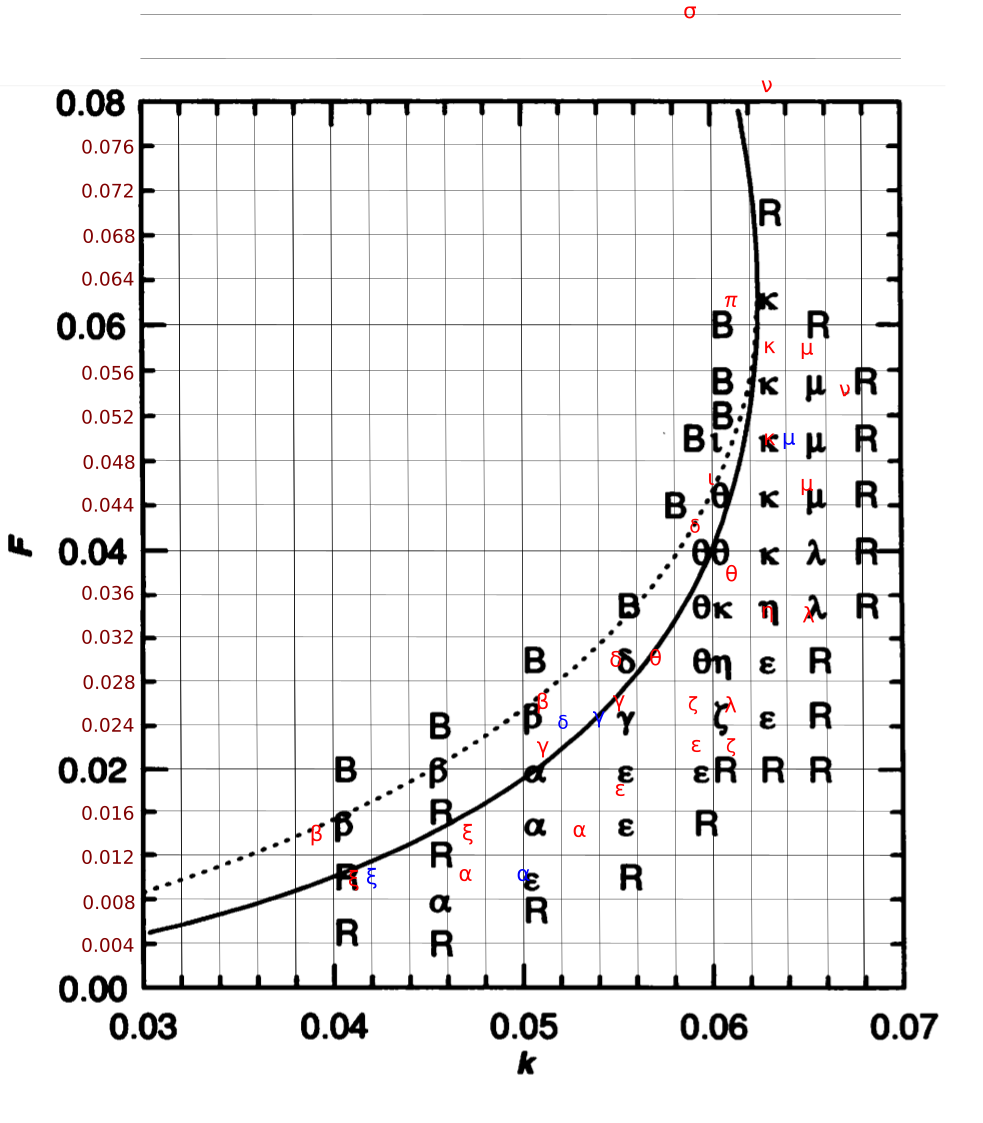
\includegraphics[width=5cm]{images/openbc/drawing.png}
\end{center}

The prescribed traction on the leftt boundary is
\[
{\vec t}={\bm \sigma}\cdot {\vec n}=
\left(
\begin{array}{cc}
-p_{bc} & 0 \\
0 & -p_{bc}
\end{array}
\right)
\cdot
\left(
\begin{array}{c}
-1 \\ 0
\end{array}
\right)
=
\left(
\begin{array}{c}
p_{bc} \\ 0
\end{array}
\right)
\]
The integral on the side of the element is then 
\[
\int_\Gamma \bN_i {\vec t} \; dS
\]
for $i=1,2,3,4$, which yields the following elemental rhs vector:
\[
\vec{F}_{el}=
\int_{\Gamma_{14}} 
\left(
\begin{array}{c}
\bN_1(x,y) t_x(x,y)\\
\bN_1(x,y) t_y(x,y)\\
\bN_2(x,y) t_x(x,y)\\
\bN_2(x,y) t_y(x,y)\\
\bN_3(x,y) t_x(x,y)\\
\bN_3(x,y) t_y(x,y)\\
\bN_4(x,y) t_x(x,y)\\
\bN_4(x,y) t_y(x,y)
\end{array}
\right)
\; dS
\]
It is worth noting that the integral takes place on the edge $\Gamma_{14}$ 
so that $\bN_2$ and $\bN_3$ are identically zero on this edge
and also $t_y=0$ 
so 
\[
\vec{F}_{el}=
\left(
\begin{array}{c}
\int_{\Gamma_{14}}  \bN_1(x,y) t_x(x,y) dS\\
0 \\
0 \\ 0 \\ 0 \\ 0 \\
\int_{\Gamma_{14}} \bN_4(x,y) t_x(x,y) dS\\
0
\end{array}
\right)
\]
If the traction (applied pressure) is constant over the element, 
then  
\[
\vec{F}_{el}=
t_x
\left(
\begin{array}{c}
\int_{\Gamma_{14}}  \bN_1(x,y)  dS\\
0 \\
0 \\ 0 \\ 0 \\ 0 \\
\int_{\Gamma_{14}} \bN_4(x,y)  dS\\
0
\end{array}
\right)
=
t_x
\left(
\begin{array}{c}
\int_{y_1}^{y_4} \bN_1(x,y) dy\\
0 \\
0 \\ 0 \\ 0 \\ 0 \\
\int_{y_1}^{y_4} \bN_4(x,y) dy\\
0
\end{array}
\right)
=
\frac{t_x h_y}{2}
\left(
\begin{array}{c}
1 \\
0 \\
0 \\ 0 \\ 0 \\ 0 \\
1 \\
0
\end{array}
\right)
\]
where $h_y$ is the height of the element along the segment. 



On the right boundary, we have $\bN_2=0$ and $\bN_3=0$, and since $t_y=0$ then 
the corresponding additional elemental right hand side vector writes:
\[
\vec{F}_{el} =
-\frac{t_x h_y}{2}
\left(
\begin{array}{c}
0\\
0\\
1 \\
0\\
1 \\
0\\
0\\
0
\end{array}
\right)
\] 

In the case where the traction is not constant over the edge, a numerical quadrature rule 
must be employed to integrate $\int_\Gamma \bN_i t_x dS$.



%....................................................................
\subsection{Three-dimensional case - $Q_1 \times P_0$ elements}

The right hand side is $ndof \times ndim = 8\times 3 = 24$ long. 

\begin{center}
\includegraphics[width=5.5cm]{images/openbc/drawing3D.png}
\end{center}

\begin{itemize}
\item The face $r=-1$ is made of nodes 1,4,5,8, so $\vec{n}=(-1,0,0)$.
Since $t_y=0$ and $t_z=0$ and $\bN_2=\bN_3=\bN_6=\bN_7$ on this face:
{\tiny
\[
\vec{F}_{el}=
\int_{\Gamma_{1458}} 
\left(
\begin{array}{c}
\bN_1(x,y,z) t_x(x,y,z)\\
\bN_1(x,y,z) t_y(x,y,z)\\
\bN_1(x,y,z) t_z(x,y,z)\\
\bN_2(x,y,z) t_x(x,y,z)\\
\bN_2(x,y,z) t_y(x,y,z)\\
\bN_2(x,y,z) t_z(x,y,z)\\
\bN_3(x,y,z) t_x(x,y,z)\\
\bN_3(x,y,z) t_y(x,y,z)\\
\bN_3(x,y,z) t_z(x,y,z)\\
\bN_4(x,y,z) t_x(x,y,z)\\
\bN_4(x,y,z) t_y(x,y,z)\\
\bN_4(x,y,z) t_z(x,y,z)\\
\bN_5(x,y,z) t_x(x,y,z)\\
\bN_5(x,y,z) t_y(x,y,z)\\
\bN_5(x,y,z) t_z(x,y,z)\\
\bN_6(x,y,z) t_x(x,y,z)\\
\bN_6(x,y,z) t_y(x,y,z)\\
\bN_6(x,y,z) t_z(x,y,z)\\
\bN_7(x,y,z) t_x(x,y,z)\\
\bN_7(x,y,z) t_y(x,y,z)\\
\bN_7(x,y,z) t_z(x,y,z)\\
\bN_8(x,y,z) t_x(x,y,z)\\
\bN_8(x,y,z) t_y(x,y,z)\\
\bN_8(x,y,z) t_z(x,y,z)
\end{array}
\right)
\; dS
=
\int_{\Gamma_{1458}} 
\left(
\begin{array}{c}
\bN_1(x,y,z) t_x\\
0 \\
0 \\
0\\
0\\
0\\
0\\
0\\
0\\
\bN_4(x,y,z) t_x\\
0\\
0\\
\bN_5(x,y,z) t_x\\
0\\
0\\
0\\
0\\
0\\
0\\
0\\
0\\
\bN_8(x,y,z) t_x\\
0 \\
0
\end{array}
\right)
\; dS
=
t_x
\left(
\begin{array}{c}
\int_{\Gamma_{1458}} \bN_1(x,y,z) dS\\ 
0\\
0\\
0\\
0\\
0\\
0\\
0\\
0\\
\int_{\Gamma_{1458}} \bN_4(x,y,z) dS\\ 
0\\
0\\
\int_{\Gamma_{1458}} \bN_5(x,y,z) dS\\
0\\
0\\
0\\
0\\
0\\
0\\
0\\
0\\
\int_{\Gamma_{1458}}  \bN_8(x,y,z) dS\\
0\\
0
\end{array}
\right)
=
\frac{h_yh_y t_x}{4}
\left(
\begin{array}{c}
1 \\
0\\
0\\
0\\
0\\
0\\
0\\
0\\
0\\
1\\
0\\
0\\
1\\
0\\
0\\
0\\
0\\
0\\
0\\
0\\
0\\
1\\
0\\
0
\end{array}
\right)
\]
}


\item
The face $r=+1$ is made of nodes 2,3,6,7, so $\vec{n}=(1,0,0)$.
so the non-zero terms are in positions $(4,7,16,19)$.

\item
The face $s=-1$ is made of nodes 1,2,5,6, so $\vec{n}=(0,-1,0)$.
so the non-zero terms are in positions $(2,5,14,17)$.

\item
The face $s=+1$ is made of nodes 3,4,7,8, so $\vec{n}=(0,+1,0)$.
so the non-zero terms are in positions $(8,11,20,23)$.

\end{itemize}


%.................................................................
\subsection{Two-dimensional case - $Q_2 \times Q_1$ elements}

We here too assume that we wish to prescribe a traction on the sides of a 2D domain
which are aligned with the vertical axis.

\subsubsection{constant traction}

It is not fundamentally different, except that the element counts 9 nodes, 
so the vector is $9\times 2=18$ long. 
The internal numbering of the nodes is as follows:
\begin{verbatim}
 velocity    pressure
 3---6---2   3-------2
 |       |   |       |
 7   8   5   |       |
 |       |   |       |
 0---4---1   0-------1
\end{verbatim}

On the left boundary nodes 0,3,7 are involved while on the right 
boundary nodes 1,2,5 are.
Assuming once again $t_x$ constant over the edge and $t_y=0$, we
have on the left side:

\[
\vec{F}_{el}=
\int_{\Gamma_{073}} 
\left(
\begin{array}{c}
\bN_0(x,y) t_x(x,y)\\
\bN_0(x,y) t_y(x,y)\\
\bN_1(x,y) t_x(x,y)\\
\bN_1(x,y) t_y(x,y)\\
\bN_2(x,y) t_x(x,y)\\
\bN_2(x,y) t_y(x,y)\\
\bN_3(x,y) t_x(x,y)\\
\bN_3(x,y) t_y(x,y)\\
\bN_4(x,y) t_x(x,y)\\
\bN_4(x,y) t_y(x,y)\\
\bN_5(x,y) t_x(x,y)\\
\bN_5(x,y) t_y(x,y)\\
\bN_6(x,y) t_x(x,y)\\
\bN_6(x,y) t_y(x,y)\\
\bN_7(x,y) t_x(x,y)\\
\bN_7(x,y) t_y(x,y)\\
\bN_8(x,y) t_x(x,y)\\
\bN_8(x,y) t_y(x,y)
\end{array}
\right)
dS
=
t_x 
\left(
\begin{array}{c}
\int_{\Gamma_{073}} \bN_0(x,y) dS\\
0 \\ 0 \\ 0 \\ 0 \\ 0 \\
\int_{\Gamma_{073}} \bN_3(x,y) dS \\
0 \\ 0 \\ 0 \\ 0 \\ 0 \\ 0 \\ 0 \\
\int_{\Gamma_{073}}  \bN_7(x,y) dS \\
0 \\ 0 \\ 0
\end{array}
\right)
=
t_x  \frac{h_y}{2}
\left(
\begin{array}{c}
\int_{-1}^{+1} \bN_0(r=-1,s) ds\\
0 \\ 0 \\ 0 \\ 0 \\ 0 \\
\int_{-1}^{+1} \bN_3(r=-1,s) ds \\
0 \\ 0 \\ 0 \\ 0 \\ 0 \\ 0 \\ 0 \\
\int_{-1}^{+1}  \bN_7(r=-1,s) ds \\
0 \\ 0 \\ 0
\end{array}
\right)
\]
We then compute
\begin{eqnarray}
\int_{-1}^{+1} \bN_0(r=-1,s) ds 
&=& \int_{-1}^{+1} \frac{1}{2}s(s-1) ds = \frac{1}{3} \\
\int_{-1}^{+1} \bN_3(r=-1,s) ds 
&=& \int_{-1}^{+1} \frac{1}{2}s(s+1) ds = \frac{1}{3} \\
\int_{-1}^{+1} \bN_7(r=-1,s) ds 
&=& \int_{-1}^{+1} (1-s^2) ds = \frac{4}{3} 
\end{eqnarray}
Note that the sum of the three terms is 2, as expected: on the edge
we have $\bN_0+\bN_3+\bN_7 =1$ so that the integral of the sum over the 
interval [-1,1] yields 2. Finally 
\[
\vec{F}_{el}
=
\frac{t_x  h_y}{6}
\left(
\begin{array}{c}
1 \\
0 \\
0 \\
0 \\
0 \\
0 \\
1 \\
0 \\
0 \\
0 \\
0 \\
0 \\
0 \\
0 \\
4 \\
0 \\
0 \\
0
\end{array}
\right)
\]
This is implemented in \stone 61, 64, 146, 148.





On the right boundary, we need to compute (careful with sign when implementing!)
\[
\vec{F}_{el}=
\int_{\Gamma_{152}} 
\left(
\begin{array}{c}
\bN_0(x,y) t_x(x,y)\\
\bN_0(x,y) t_y(x,y)\\
\bN_1(x,y) t_x(x,y)\\
\bN_1(x,y) t_y(x,y)\\
\bN_2(x,y) t_x(x,y)\\
\bN_2(x,y) t_y(x,y)\\
\bN_3(x,y) t_x(x,y)\\
\bN_3(x,y) t_y(x,y)\\
\bN_4(x,y) t_x(x,y)\\
\bN_4(x,y) t_y(x,y)\\
\bN_5(x,y) t_x(x,y)\\
\bN_5(x,y) t_y(x,y)\\
\bN_6(x,y) t_x(x,y)\\
\bN_6(x,y) t_y(x,y)\\
\bN_7(x,y) t_x(x,y)\\
\bN_7(x,y) t_y(x,y)\\
\bN_8(x,y) t_x(x,y)\\
\bN_8(x,y) t_y(x,y)
\end{array}
\right)
dS
=
t_x 
\left(
\begin{array}{c}
0 \\ 0 \\
\int_{\Gamma_{125}} \bN_1(x,y) dS \\ 0 \\ 
\int_{\Gamma_{125}} \bN_2(x,y) dS \\ 0 \\
0 \\ 0 \\
0 \\ 0 \\ 
\int_{\Gamma_{125}} \bN_5(x,y) dS \\
0 \\ 0 \\ 
0 \\ 0 \\ 
0 \\ 0
\end{array}
\right)
=
t_x  \frac{h_y}{2}
\left(
\begin{array}{c}
0 \\ 0 \\
\int_{-1}^{+1} \bN_1(-1,s) ds \\ 0 \\ 
\int_{-1}^{+1} \bN_2(-1,s) ds \\ 0 \\
0 \\ 0 \\
0 \\ 0 \\
\int_{-1}^{+1} \bN_5(-1,s) ds \\
0 \\ 0 \\
0 \\ 0 \\
0 \\ 0 
\end{array}
\right)
=
\frac{t_x h_y}{6}
\left(
\begin{array}{c}
0 \\ 0 \\
1 \\ 0 \\
1 \\ 0 \\
0 \\ 0 \\
0 \\ 0 \\
4 \\ 0 \\
0 \\ 0 \\
0 \\ 0 \\
0 \\ 0
\end{array}
\right)
\]

%---------------------------------------------------------------
\subsubsection{linear traction}

Let us now turn to the case where the traction we wish to apply 
on the boundary is not piecewise constant but linear.
We set $t_x(y)=ay+b$, so that on the right side (nodes, 1,2,5), we have to compute

\begin{eqnarray}
\int_{\Gamma_{125}} \bN_1(x,y) t_x(y) dS 
&=&\int_{\Gamma_{125}} \bN_1(x,y) (ay+b) dy \nn\\
&=&\frac{h_y}{2} \int_{-1}^1 \bN_1(r=1,s) [ay(s)+b] ds \nn
\end{eqnarray}
We have 
\[
s(y)=\frac{2}{h_y}(y-y_1)-1 
\qquad
\text{or}
\qquad
y(s)= \frac{h_y}{2}(s+1) +y_1
\]
and
\[
\bN_1(r,s) 
= \frac{1}{2}r(r+1)\frac{1}{2}s(s-1)
\qquad
\Rightarrow
\qquad
\bN_1(r=1,s) 
= \frac{1}{2}1(1+1)\frac{1}{2}s(s-1) 
= \frac{1}{2}s(s-1) 
\]
Then
\begin{eqnarray}
\int_{\Gamma_{125}} \bN_1(x,y) t_x(y) dS 
&=&\frac{h_y}{2} \int_{-1}^1 \bN_1(r=1,s) \left[ a \left(\frac{h_y}{2}(s+1) +y_1\right) +b \right] ds \nn\\
&=&\frac{h_y}{2} \int_{-1}^1 \frac12 s(s-1) \left[ a \left(\frac{h_y}{2}(s+1) +y_1\right) +b \right] ds \nn\\
&=&\frac{h_y}{4} \int_{-1}^1 s(s-1) \left[ \frac{a h_y}{2}(s+1) + (ay_1+b) \right] ds \nn\\
&=& \frac{h_y}{4} \left[
\frac{a h_y}{2} \int_{-1}^1 s(s-1) (s+1)  ds 
+(ay_1+b) \int_{-1}^1 s(s-1)   ds 
\right] \nn\\
&=& \frac{h_y}{4} 
\frac{a h_y}{2} \underbrace{\int_{-1}^1 s(s^2-1)  ds}_{=0} 
+\frac{h_y}{4} (ay_1+b) \underbrace{\int_{-1}^1 s(s-1)   ds}_{=2/3} \nn\\
&=& \frac{h_y}{6} (ay_1+b)
\end{eqnarray}

Let us now turn to $\bN_2$:
\[
\bN_2(r,s) = \frac12 r(r+1) \frac12 s(s+1)
\qquad
\Rightarrow
\qquad
\bN_2(r=1,s) = \frac12 s(s+1)
\]
Then
\begin{eqnarray}
\int_{\Gamma_{125}} \bN_2(x,y) t_x(y) dS 
&=&\frac{h_y}{2} \int_{-1}^1 \bN_2(r=1,s) \left[ a \left(\frac{h_y}{2}(s+1) +y_1\right) +b \right] ds \nn\\
&=&\frac{h_y}{2} \int_{-1}^1 \frac12 s(s+1) \left[ a \left(\frac{h_y}{2}(s+1) +y_1\right) +b \right] ds \nn\\
&=&\frac{h_y}{4} \int_{-1}^1 s(s+1) \left[ \frac{a h_y}{2}(s+1) + (ay_1+b) \right] ds \nn\\
&=& \frac{h_y}{4} \left[
\frac{a h_y}{2} \int_{-1}^1 s(s+1) (s+1)  ds 
+(ay_1+b) \int_{-1}^1 s(s+1)   ds 
\right] \nn\\
&=& \frac{h_y}{4} 
\frac{a h_y}{2} \underbrace{\int_{-1}^1 s(s+1)^2  ds}_{=4/3} 
+\frac{h_y}{4} (ay_1+b) \underbrace{\int_{-1}^1 s(s+1)  ds}_{=2/3} \nn \\
&=& \frac{h_y}{6} \left( a h_y + ay_1+b   \right)
\end{eqnarray}



And finally let us turn to $\bN_5$:
\[
\bN_5(r,s) = \frac12 r(r+1) (1-s^2)
\qquad
\Rightarrow
\qquad
\bN_5(r=1,s) =  (1-s^2)
\]
then
\begin{eqnarray}
\int_{\Gamma_{125}} \bN_5(x,y) t_x(y) dS 
&=&\frac{h_y}{2} \int_{-1}^1 \bN_2(r=1,s) \left[ a \left(\frac{h_y}{2}(s+1) +y_1\right) +b \right] ds \nn\\
&=&\frac{h_y}{2} \int_{-1}^1  (1-s^2) \left[ a \left(\frac{h_y}{2}(s+1) +y_1\right) +b \right] ds \nn\\
&=&\frac{h_y}{2} \int_{-1}^1 (1-s^2) \left[ \frac{a h_y}{2}(s+1) + (ay_1+b) \right] ds \nn\\
&=& \frac{h_y}{2} \left[
\frac{a h_y}{2} \int_{-1}^1 (1-s^2) (s+1)  ds 
+(ay_1+b) \int_{-1}^1 (1-s^2)   ds 
\right] \nn\\
&=& \frac{h_y}{2} \frac{a h_y}{2} \underbrace{\int_{-1}^1 (1-s^2)(1+s)  ds}_{=4/3} 
+\frac{h_y}{2} (ay_1+b) \underbrace{\int_{-1}^1 (1-s^2)  ds}_{=4/3} \nn \\
&=& \frac{h_y}{6} \left( 2 a h_y + 4ay_1+4 b   \right)
\end{eqnarray}
Note that by setting $a=0$ and $b=t_x$ we recover the expressions above for a 
piecewise constant value.

If we know $p_1$ and $p_2$ (say, for example that the lithostatic pressure has been computed on these nodes
and we wish to prescribe it on the side) then 
\[
t_y=ay+b = \underbrace{\frac{p_2-p_1}{y_2-y_1}}_{=a} y + \underbrace{p_1-\frac{p_2-p_1}{y_2-y_1} y_1}_{=b}
\]

On the left side (nodes 0,7,3), we have to compute
\begin{eqnarray}
\int_{073} \bN_0(x,y) (ay+b) dS
&=& \frac{h_y}{2} \int_{-1}^{+1} \bN_0(r=-1,s) [ay(s)+b] ds \\
\int_{073} \bN_3(x,y) (ay+b) dS 
&=& \frac{h_y}{2} \int_{-1}^{+1} \bN_3(r=-1,s) [ay(s)+b] ds  \\
\int_{073} \bN_7(x,y) (ay+b) dS 
&=& \frac{h_y}{2} \int_{-1}^{+1} \bN_7(r=-1,s) [ay(s)+b] ds  
\end{eqnarray}
with 
\begin{align}
\bN_0 (r,s) &= \frac12 r(r-1) \frac12 s(s-1)  \rightarrow  \bN_0 (-1,s) &=  \frac12 s(s-1) \nonumber\\  
\bN_3 (r,s) &= \frac12 r(r-1) \frac12 (1-s^2) \rightarrow  \bN_3 (-1,s) &=  (1-s^2) \nonumber\\
\bN_7 (r,s) &= \frac12 r(r-1) \frac12 s(s+1)  \rightarrow  \bN_7 (-1,s) &=  \frac12 s(s+1) \nonumber
\end{align}


If we know $p_0$ and $p_3$ then 
\[
t_x=ay+b = \underbrace{\frac{p_3-p_0}{y_3-y_0}}{=a} y + \underbrace{p_0-\frac{p_3-p_0}{y_3-y_0} y_0}_{=b}
\]










%\begin{center}
%\includegraphics[width=4cm]{FEM/openbc/openbc1.png}
%\includegraphics[width=4cm]{FEM/openbc/openbc2.png}\\
%{\small Example of a Stokes sphere sinking when 
%both $y=0$ and $y=L_y$ walls are subjected to
%open boundary conditions.}
%\end{center}


%.................................................................
\subsection{Two-dimensional case - Linear triangle elements}

Let us assume we want to apply a stress on the face 13 of the following element:
\begin{verbatim}
   1-------------3
    \           /
     \         /
      \       /
       \     /
        \   /
         \ /
          2
\end{verbatim}

The integral on the side of the element is $\int_\Gamma \bN_i {\vec t} \; dS$
for $i=1,2,3$, which yields the following elemental rhs vector:
\[
\vec{F}_{el}=
\int_{\Gamma_{13}} 
\left(
\begin{array}{c}
\bN_1(x,y) t_x(x,y)\\
\bN_1(x,y) t_y(x,y)\\
\bN_2(x,y) t_x(x,y)\\
\bN_2(x,y) t_y(x,y)\\
\bN_3(x,y) t_x(x,y)\\
\bN_3(x,y) t_y(x,y)
\end{array}
\right)
\; dS
=
\int_{\Gamma_{13}} 
\left(
\begin{array}{c}
0\\
\bN_1(x,y) t_y(x,y)\\
0\\
0\\
0\\
\bN_3(x,y) t_y(x,y)
\end{array}
\right)
\; dS
\]
since $t_x=0$ and there function $\bN_2$ will be zero on the edge.

We also arbitrarily set $y_1=y_3=0$. We have seen in Section~\ref{shpfct2d} that 
the basis functions (expressed as a function of the real coordinates $x,y$) 
for a linear triangle are given by:
\begin{eqnarray}
\bN_1(x,y) &=& \frac{1}{D}[(x_2y_3-x_3y_2) + (y_2-y_3)x + (x_3-x_2)y] \nn\\
\bN_2(x,y) &=& \frac{1}{D}[(x_3y_1-x_1y_3) + (y_3-y_1)x + (x_1-x_3)y] \nn\\
\bN_3(x,y) &=& \frac{1}{D}[(x_1y_2-x_2y_1) + (y_1-y_2)x + (x_2-x_1)y] \nn
\end{eqnarray}
with 
\[
D = 
\left|
\begin{array}{ccc}
1 & x_1 & y_1 \\
1 & x_2 & y_2 \\
1 & x_3 & y_3 
\end{array}
\right|
=
\left|
\begin{array}{ccc}
1 & x_1 & 0 \\
1 & x_2 & y_2 \\
1 & x_3 & 0 
\end{array}
\right|
=
-x_3y_2+x_1y_2
= y_2(x_1-x_3)
\]


\begin{eqnarray}
\int_{x_1}^{x_3} \bN_1(x,y=0) dx 
&=& \frac{1}{D} \int_{x_1}^{x_3} [(x_2y_3-x_3y_2) + (y_2-y_3)x ] \nn\\
&=& \frac{1}{D} \int_{x_1}^{x_3} [-x_3y_2 + y_2 x ] \qquad \text{since} y_1=y_3=0 \nn\\
&=& \frac{y_2}{D} \int_{x_1}^{x_3} (-x_3 +  x ) dx \nn\\
&=& \frac{y_2}{y_2(x_1-x_3)  } [ -x_3 x + \frac{1}{2}x^2]_{x_1}^{x_3} \nn\\ 
&=& \frac{1}{x_1-x_3 } [ -x_3 (x_3-x_1) + \frac{1}{2}(x_3^2-x_1^2)] \nn\\
&=& \frac{1}{x_1-x_3 } [ x_3 (x_1-x_3) + \frac{1}{2}(x_3-x_1)(x_3+x_1)] \nn\\
&=&  x_3 - \frac{1}{2}(x_3+x_1) \nn\\
&=&  \frac{1}{2} (x_3-x_1) \\
\int_{x_1}^{x_3} \bN_3(x,y=0) dx
&=& \frac{1}{D} \int_{x_1}^{x_3}    [(x_1y_2-x_2y_1) + (y_1-y_2)x ] dx \nn\\
&=& \frac{1}{D} \int_{x_1}^{x_3}    [x_1y_2 - y_2x ] dx \nn\\
&=& \frac{y_2}{D} \int_{x_1}^{x_3}    [x_1 - x ] dx \nn\\
&=& \frac{y_2}{y_2(x_1-x_3) } [x_1 x - \frac{1}{2} x^2]_{x_1}^{x_3}  \nn\\
&=& \frac{1}{x_1-x_3} [x_1 (x_3-x_1) - \frac{1}{2} (x_3^2-x_1^2)] \nn\\
&=& -x_1  + \frac{1}{2} (x_3+ x_1) \nn\\
&=& \frac{1}{2}( x_3 -x_1 )
\end{eqnarray}
Finally
\[
\vec{F}_{el}=
\frac{h t_y}{2}
\left(
\begin{array}{c}
0\\
1 \\
0\\
0\\
0\\
1 
\end{array}
\right)
\]





